% Single laser work
\documentclass[10pt,twocolumn,letterpaper]{article}

\usepackage{graphicx} % for \includegraphics[scale=•]{•}

\begin{document}
\title{Stage Oriented Design of an Intersection Management System Based on Laser Scanner Data}

\author{Gustavo Velasco-Hernandez, Eduardo Caicedo-Bravo \\
Universidad del Valle\\
{\tt\small velasco.gustavo@correounivalle.edu.co, eduardo.caicedo@correounivalle.edu.co}
% For a paper whose authors are all at the same institution,
% omit the following lines up until the closing ``}''.
% Additional authors and addresses can be added with ``\and'',
% just like the second author.
% To save space, use either the email address or home page, not both
}

\maketitle

\begin{abstract}
In this work is described a stage-oriented design of an intersection management system based on a laser scanner sensor. After an introduction of the use of laser scanners in traffic monitoring, four stages are defined in the process flow of such a systems: preprocessing, feature analysis, pattern recognition and situation assesment. Then, an example implementation using a laser scanner dataset is presented.
\end{abstract}

\section{Introduction}
Lorem ipsum dolor sit amet, mei vulputate argumentum an, usu vidit labitur ancillae et, quot accusamus cum et. Recteque dissentiet vim ea, est virtute alterum ea, mei dico scribentur in. Et eam paulo soleat graeci. Ius viderer habemus scriptorem ut, no mea vocibus albucius. Sed no perpetua suscipiantur, pro diam nullam erroribus id. Pro labore audire et, tale eligendi mediocrem his cu, te sonet adipisci ius. Exerci regione noluisse mea no, no usu mazim mediocrem assentior, at audire volumus eam. Soluta oporteat recteque ut ius, nam an sumo solet facilisis, rebum aeque eam et. Pri quot graece in. Dictas liberavisse.

\section{Stages Definition}
In the designing of an IMS, there are four main stages that have to be performed from the data source to final output: preprocessing, feature analysis, pattern recognition and situation assessment.

The aim of the first stage is to extract data of interest from the raw sensor information, using filtering and background subtraction techniques to get the foreground of the scene, remove noise and irrelevant data. Spatio-temporal alignment of data is also performed in this stage. In the second stage, the objective is to identify elements within the foreground and extract relevant features of them. The third stage receives the set of features from the previous stage and performs recognition and classification tasks. Also, tracking and prediction of objects' state is performed based on historic information. In the fourth stage, object behaviour and inter-objects interaction are analysed to identify context and detect situation or events of interest.

The output of the fourth stage could be delivered to an optional fifth stage of decision and control, to a human operator, or to a traffic agent or institution, to take immediate actions on traffic control, issue traffic tickets, warn drivers about possible incidents or improve transportation policies in a long-term basis. In figure \ref{proc_stages}, previously described stages are depicted, and also is shown how the data volume is reduced while data meaning increases in the last stages.

\begin{figure}[ht!]
\centering
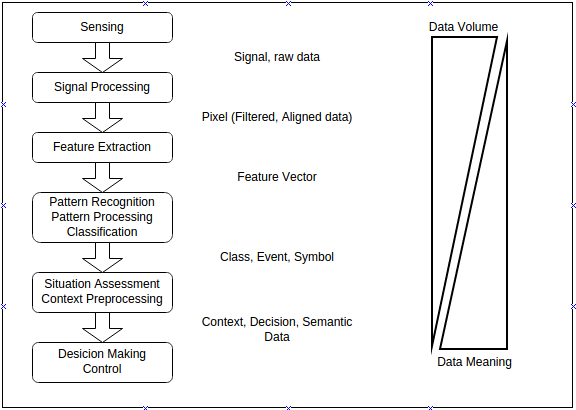
\includegraphics[scale=0.35]{../fig/3/proc_stages.png}
\caption{Dataflow through processing stages in an IMS.}
\label{proc_stages}
\end{figure}

Different tasks could be performed in each aforementioned stages, as is referred in figure \ref{proc_stages_tasks}. Below there is a description of common concepts and techniques associated with each of these tasks.

\begin{figure}[ht!]
\centering
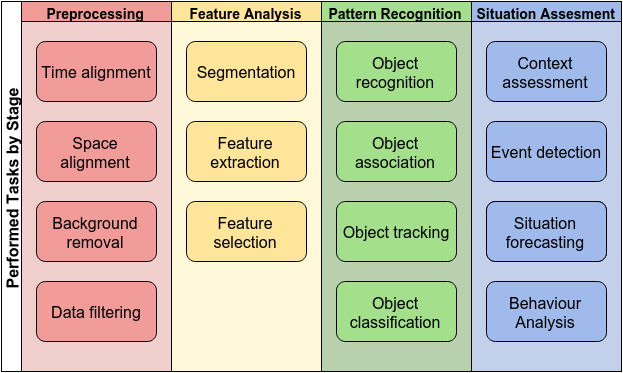
\includegraphics[scale=0.35]{../fig/3/processing_stages_and_tasks.png}
\caption{Processing stages and tasks performed.}
\label{proc_stages_tasks}
\end{figure}
\subsection{Preprocessing}

 In the preprocessing stage raw data from sensor is received and the purpose is to enhance this data through filtering noise, removing outliers and discarding corrupted data. Also, in order to extract meaningful information, background removal techniques are applied in this stage. For doing this, a background model should be generated. One typical approach to generate a background model is to use a threshold to determine if certain measure corresponds to background or foreground. This threshold is computed based on a peak value found in histogram of the measure within a time window. Another approach consist in describe the data using a probability distribution function, using maximum likelihood estimation, commonly of a gaussian model.
 
Sometimes, the threshold technique is enough for modeling static backgrounds like walls, buildings or ground. But in other cases, it could be found a non-stable background, for example, when there exist moving vegetation or object borders, and a mixture of models may retrieve a better representation of the data instead.

\subsection{Feature Analysis}

After obtaining the foreground of the scene, it is needed to extract relevant points that could represent objects of interest. Clustering is used to group points that belong to the same object, specially algorithms where estimated number of cluster is not needed. 


\subsection{Pattern Recognition}
\subsection{Situation Assesment}

\section{Laser-based System Implementation}

\subsection{Dataset}
 The dataset used for this work was provided by POSS research group and was used for \cite{Zhao2009}. The dataset consist of ten minutes of laser scanner raw data from six sensors arranged horizontally over an intersection near Peking University. Background model and calibration data for each laser scanner is also provided. Additionally, dataset contains trajectory info of objects in the scene, generated by their algorithm.
 
\subsection{Preprocessing}

As mentioned before, the dataset provides a background model for each laser scanner. This model was generated using a histogram of each sampling angle of scanning, then a peak is found indicating a motionless object, considered as background. With the peak values at all sampling angles the background model is obtained. Now, when a new frame comes from the laser scanner, the measure at certain angle is compared with the peak value associated with that angle. If the difference is larger than a given threshold, the measured value is considered to belong to a moving object at the intersection.

\subsection{Feature Analysis}

With the set of points marked as foreground, clustering is performed to identify the set of points belonging to the same object. The algorithm used in this implementation is DBSCAN, which stands for Density-Based Spatial Clustering of Applications with Noise. This algorithm does not need an estimated number of clusters as input, instead of this, it requires only two parameters: a minimum number of points per cluster, m, and a neighbourhood measure, $\epsilon$. A detailed description of the algorithm, can be found in \cite{Ester96}.
\subsection{Pattern Recognition}
\subsection{Situation Assesment}

\section{Results}

\section{Conclusions and Future Work}

{\small
\bibliographystyle{plain}
\bibliography{../bibliography}
}

\end{document}